\documentclass[letter,12pt]{article}
\usepackage{epsfig,latexsym,amsmath,amssymb,epic,eepic,psfrag,subfigure,float,euscript,array}
\usepackage[latin1]{inputenc}
\usepackage{standalone}
\usepackage{tikz,pgf,pgfplots}
\usepackage[margin=2.5cm]{geometry}

\newenvironment{exercise}[1][Uppgift]{\begin{trivlist} \item[\hskip
    \labelsep {\stepcounter{exerctr}\bfseries #1
      \arabic{exerctr}}]}{\end{trivlist}\vspace{10mm}}

\newcounter{exerctr}
\newcounter{abcctr}[exerctr]

\newcommand{\abc}{\noindent\vspace{1mm}\\ {\bf
    \stepcounter{abcctr}(\alph{abcctr})\ }}
\newcommand{\bbm}{\begin{bmatrix}}
\newcommand{\ebm}{\end{bmatrix}}
\newcommand{\point}[1]{\hfill {\bf (#1p)}\\ \vspace{-5mm}}
\newcommand{\ctrb}{\EuScript{S}}
\newcommand{\Lap}{\mathcal{L}}
\newcommand{\obsv}{\EuScript{O}}
\newcommand{\realdel}[1]{\text{Re}\left\{#1\right\}}
\newcommand{\imagdel}{\text{Im}}
\newcommand{\bC}{\mathbb{C}}
\newcommand{\bR}{\mathbb{R}}
\newcommand{\bmpv}{\begin{minipage}[t]}
\newcommand{\bmps}{\begin{minipage}[t]{45mm}}
\newcommand{\bmpm}{\begin{minipage}[t]{90mm}}
\newcommand{\bmpl}{\begin{minipage}[t]{\textwidth}}
\newcommand{\emp}{\end{minipage}}
\newcommand*{\zethree}{\big(z - \mexp{-3h}\big)}
\newcommand*{\mexp}[1]{\ensuremath{\mathrm{e}^{#1}}}

\newcommand*\circled[1]{\tikz[baseline=(char.base)]{
            \node[shape=circle,draw,inner sep=2pt] (char) {#1};}}

\addtolength{\topmargin}{-1cm}
\textheight 23.5cm
%\oddsidemargin 0.61cm
%\evensidemargin 0.61cm


\title{Computerized control final exam (26\%)}
\author{Kjartan Halvorsen}

\begin{document}

\maketitle


\begin{description}
\item[Time] 2016-11-25 17:35 - 19:00
\item[Place] 5211
\item[Permitted aids] The single colored page with your own notes, table of transforms, calculator
\end{description}

All answers should be readable and well motivated (if nothing else is written). Solutions/motivations should be written on the provided spaces in this exam. Use the last page if more space is needed.

\begin{center}
{\Large Good luck!} \\
\end{center}

\noindent
\fbox{
\bmpl
{\bf Matricula and name:}\\
\vspace*{30mm}
\emp}

\clearpage

%-----------------------------------------------------------------


\subsection*{Problem 1 (50p)}
% Cancelling zero of double integrator - See example 3.15
The double-integrator
\begin{center}
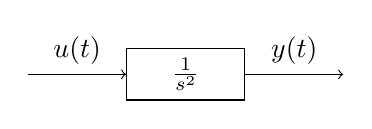
\begin{tikzpicture}[block/.style={rectangle, draw, minimum width=15mm},]
  \node[block] (plant) {$\frac{1}{s^2}$};
  \draw[->] (plant) ++ (-2cm,0) -- node [above] {$u(t)$} (plant);
  \draw[<-] (plant) ++ (2cm,0) -- node [above] {$y(t)$} (plant);
\end{tikzpicture}
\end{center}
is a common model in physical systems where force (or torque) is the input and the position (or angle) is the output, and where the load is purely inertial (no friction, damping or elastic elements).

Zero-order-hold sampling of the double integrator with sampling period $h=1$ gives the discrete-time model
\begin{equation}
 y(k) = \frac{(q+1)}{2(q-1)^2} u(k) 
\label{eq:doubleint}
\end{equation}

\subsubsection*{(a)}
Write the system in \eqref{eq:doubleint} as a \emph{difference equation}.

\noindent
\fbox{
\bmpl
{\bf Solution:}\\
\vspace*{60mm}
\emp}

\subsubsection*{(b)}
The plant is to be controlled by the two-degrees-of-freedom controller illustrated in figure~\ref{fig:feedback}.
\begin{figure}
\begin{center}
     \begin{tikzpicture}[scale = 0.8, node distance=25mm, block/.style={rectangle, draw, minimum width=15mm}, sumnode/.style={circle, draw, inner sep=2pt}]
     
     \node[sumnode, ] (sumerr) {\tiny $\sum$};
     \node[block, left of=sumerr] (ffw) {$\frac{2z}{z+1}$};
     \node[coordinate, left of=ffw] (refinput) {};
     %\node[above of=controller, node distance=6mm] {controller};
     \node[block, right of=sumerr, node distance=30mm] (plant) {$\frac{z+1}{2(z-1)^2}$};
     \node[block, below of=plant, node distance=20mm] (ffb) {$\frac{2(2z-1)}{z+1}$};

     %\node[sumnode, right of=plant, node distance=24mm] (sum) {\tiny $\sum$};
     %\node[above of=tank, node distance=6mm] {motor};
     \node[coordinate, right of=plant, node distance=20mm] (measurement) {};
     \node[coordinate, right of=measurement, node distance=20mm] (output) {};
     %\node[coordinate, above of=sum, node distance=12mm] (disturbance) {};

     \draw[->] (refinput) -- node[above, near start] {$u_c(k)$} (ffw);
     \draw[->] (ffw) -- node[above] {} (sumerr);
     \draw[->] (sumerr) -- node[above] {$u(k)$} (plant);
     \draw[->] (plant) -- node[above, near end] {$y(k)$} (output);
     \draw[->] (measurement) |- (ffb);
     \draw[->] (ffb) -| (sumerr) node [left, pos=0.9] {$-$};

     \end{tikzpicture}
     \caption{Closed-loop system, problem 1 (b).}
     \label{fig:feedback}
   \end{center}
 \end{figure}
Show that the closed-loop system from the command signal $u_c(k)$ to the output $y(k)$ can be written
\[ Y(z) = \frac{z(z+1)}{z^2(z+1)} U_c(z) = z^{-1} U_c(z). \]

\noindent
\fbox{
\bmpl
{\bf Solution:}\\
\vspace*{140mm}
\emp}

\subsubsection*{(c)}
The controller from (b) gives the closed-loop discrete-time response
\[ y(k) = u_c(k-1) \]
which appears to be a system with very good performance, since the output follows the input perfectly with just a small delay of a single sampling period. Too good to be true? Yes, there is an important flaw with this controller, as shown in the simulation below. This is an example of hidden oscillations (oscillations in the continuous-time system that are invisible at the sampling instants).  
\begin{center}
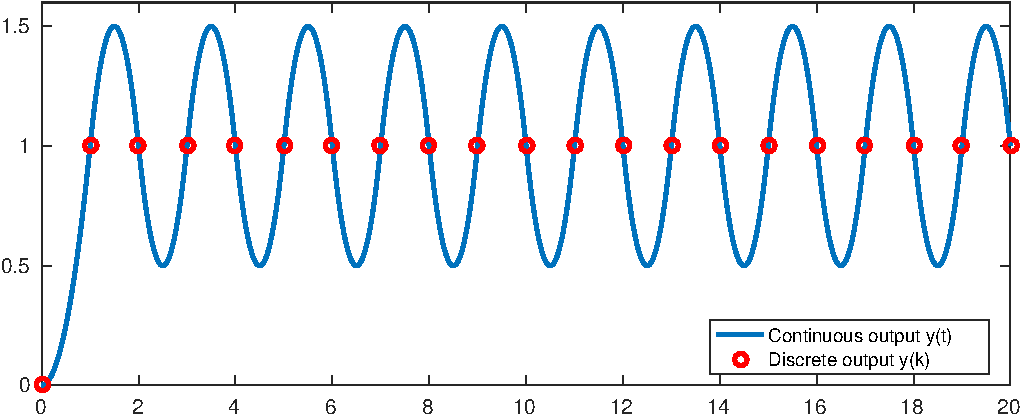
\includegraphics[width=0.7\linewidth]{p1_closed_loop_step-crop}
\end{center}

Consider the feedback part of the controller
\begin{equation}
 F_{fb}(z) = \frac{2(2z-1)}{z+1}. 
 \label{eq:feedback}
\end{equation}
Figure~\ref{fig:step} shows four step-responses. Which of these responses corresponds to the step-response from the system \eqref{eq:feedback}? Motivate!

\noindent
\fbox{
\bmpl
{\bf Answer and motivation:}\\
\vspace*{100mm}
\emp}



\begin{figure}[tp]
\begin{center}
\begin{tabular}{cc}
A & B\\
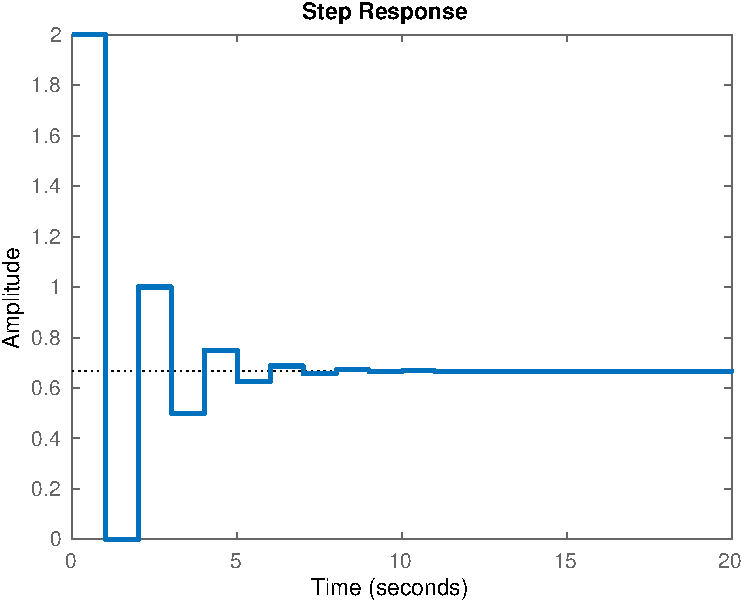
\includegraphics[width=0.4\linewidth]{step-plot-1-crop}
&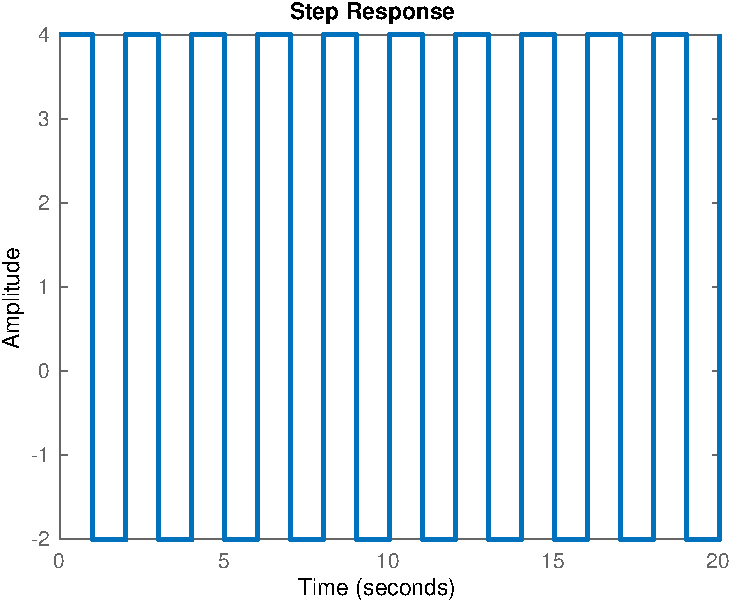
\includegraphics[width=0.4\linewidth]{step-plot-2-crop}\\
C & D\\
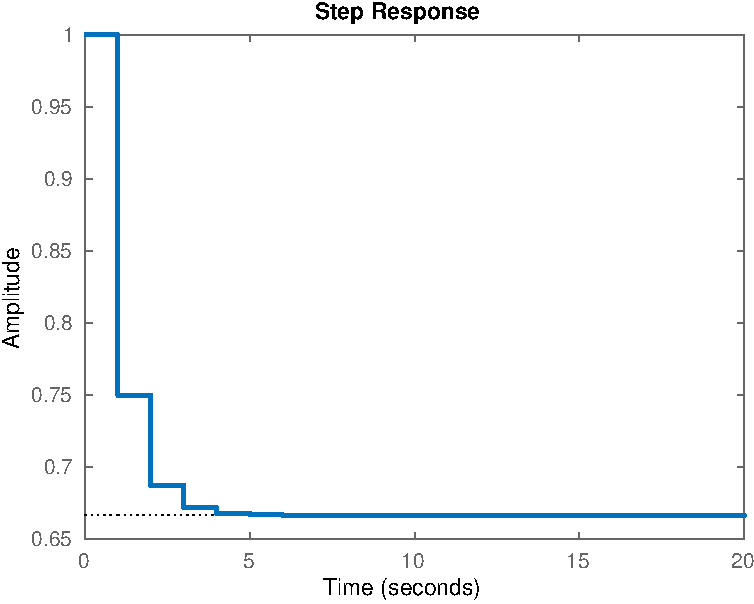
\includegraphics[width=0.4\linewidth]{step-plot-3-crop}
&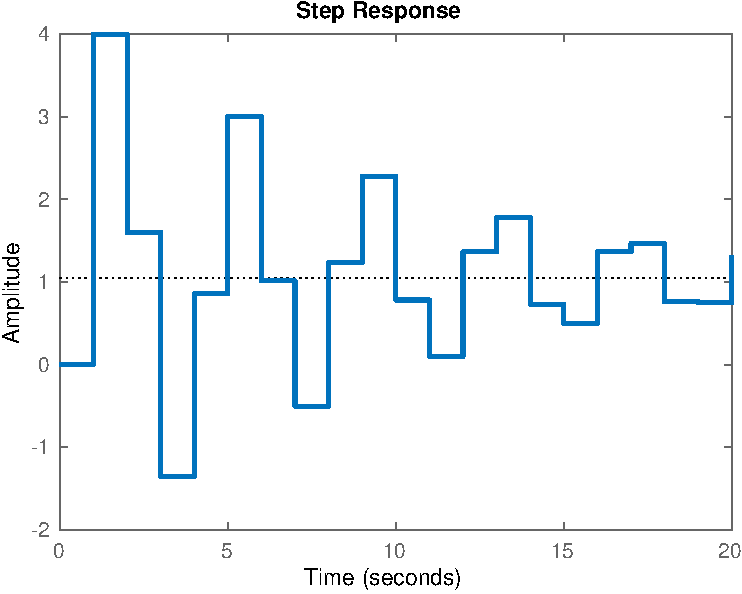
\includegraphics[width=0.4\linewidth]{step-plot-4-crop}

\end{tabular}
\caption{Step responses, problem 1 (c).}
\label{fig:step}
\end{center}
\end{figure}


\cleardoublepage

\subsection*{Problem 2 (50p)}

The double-integrator can be represented on state-space form as
\begin{equation}
\begin{split}
x(k+1) &= \bbm 1 & 1\\0 & 1\ebm x(k) + \bbm 0.5\\1\ebm u(k)\\
y(k) &= \bbm 1 & 0 \ebm u(k)
\end{split}
\end{equation}

\subsubsection*{(a)}

Show that state-space model indeed corresponds to the pulse transfer function
\[ H(z) = \frac{z+1}{2(z-1)^2}. \]

\noindent
\fbox{
\bmpl
{\bf Solution:}\\
\vspace*{120mm}
\emp}



\subsubsection*{(b)}

Determine a state feedback 
\[ u(k) = u_c(k) - k_1 x_1(k) - k_2 x_2(k) \]
which gives a closed-loop system with poles in the origin, i.e.~deadbeat control.

\noindent
\fbox{
\bmpl
{\bf Controller design:}\\
\vspace*{160mm}
\emp}



\cleardoublepage

\noindent
{\bf If necessary,} you can continue your solutions on this sheet. Mark clearly which problem the solution corresponds to.

%\end{document}

\section*{Solutions}
\subsection*{Problem 1}

\subsubsection*{(a)}

\begin{equation*}
\begin{split}
 y(k) &= \frac{(q+1)}{2(q-1)^2} u(k) \\
2(q-1)^2y(k) &= (q+1)u(k)\\
2(q^2 - 2q +1)y(k) &= (q+1)u(k)\\
2y(k+2) - 4y(k+1) + 2y(k) &= u(k+1) + u(k).
\end{split}
\end{equation*}

\subsubsection*{(b)}
Using Mason's rule (``gain of direct path to output divided by one plus the loop gain'') we get
\begin{equation}
\begin{split}
Y(z) &= \frac{ \frac{z+1}{2(z-1)^2} \cdot \frac{2z}{z+1}}{ 1 + \frac{z+1}{2(z-1)^2} \cdot \frac{2(2z-1)}{z+1}}U_c(z) \\
     &= \frac{ \frac{z}{(z-1)^2}}{1 + \frac{2z-1}{(z-1)^2} }U_c(z)\\
     &= \frac{ z }{(z-1)^2 + (2z-1)} = \frac{z}{z^2} = z^{-1} U_c(z).
   \end{split}
 \end{equation}

\subsubsection*{(c)}

The system (the feedback controller) 
\[ F_{fb}(z) = \frac{2(2z-1)}{z+1}\]
has a pole in \(z=-1\). Such a system will give time-responses with alternating positive and negative values and without decay since the pole is on the unit circle. This corresponds to step response \textbf{B}. One can also argue that all step-responses except B show stable, decaying responses.

\subsection*{Problem 2}

\subsubsection*{(a)}
Take the z-transform of the state-space system 
\begin{equation}
\begin{split}
x(k+1) &= \underbrace{\bbm 1 & 1\\0 & 1\ebm}_{\Phi} x(k) + \underbrace{\bbm 0.5\\1\ebm}_{\Gamma} u(k)\\
y(k) &= \underbrace{\bbm 1 & 0 \ebm}_{C} u(k)
\end{split}
\end{equation}

and assume the initial states to be zero to obtain
\begin{equation}
\begin{split}
zX &= \Phi X + \Gamma U\\
(zI - \Phi) X &= \Gamma U\\
X &= (zI-\Phi)^{-1}\Gamma U.
\end{split}
\end{equation}
Insert into the measurement equation to get
\[ Y = C(zI-\Phi)^{-1}\Gamma U,\]
so the pulse transfer function is given by
\begin{equation}
\begin{split}
H(z) &= C(zI-\Phi)^{-1}\Gamma = C \bbm z-1 & -1\\ 0 & z-1 \ebm^{-1}\Gamma\\
     &= C \frac{1}{(z-1)^2} \bbm z-1 & 1\\ 0 z-1 \ebm \bbm 0.5\\1\ebm 
      = \frac{1}{(z-1)^2} \bbm 1 & 0 \ebm  \bbm 0.5(z-1)+ 1\\ z-1 \ebm\\
     &= \frac{0.5z + 0.5}{(z-1)^2} = \frac{z+1}{2(z-1)^2}
   \end{split} 
 \end{equation}
 
\subsubsection*{(b)}

With the feedback \[u(k) = u_c(k) - k_1 x_1(k) - k_2 x_2(k) = u_c(k) - Kx(k) \]
inserted into the state-space model we get the closed-loop state space model
\begin{equation*}
\begin{split}
x(k+1) = \left(\Phi - \Gamma K\right)x(k) + \Gamma u_c(k)
\end{split}
\end{equation*}
which have poles given by the characteristic equation of $\Phi - \Gamma K$
\[ \det \left(zI - (\Phi - \Gamma K)\right) = 0. \] We have
\[ \Gamma K = \bbm 0.5 k_1 & 0.5 k_2\\ k_1 & k_2 \ebm \] and
\[ \Phi - \Gamma K = \bbm 1 - 0.5k_1 & 1-0.5k_2\\-k_1 & 1 - k_2 \ebm \] which gives
\begin{equation*}
\begin{split}
\det \left(zI - (\Phi - \Gamma K)\right)  &= \det \bbm z - (1 - 0.5k_1) & -(1-0.5k_2)\\-(-k_1) & z-(1 - k_2) \ebm  = \det \bbm z - 1 + 0.5k_1 & -1+0.5k_2\\k_1 & z- 1 + k_2 \ebm\\
  &= (z - 1 + 0.5k_1)(z- 1 + k_2) - (-1+0.5k_2)k_1\\
  &= z^2 + (0.5k_1 +k_2 - 2)z + (0.5k_1-1)(k_2-1) + k_1 - 0.5k_1k_2\\
  &= z^2 + (0.5k_1 + k_2 - 2)z -k_2 -0.5k_1 + 1 + k_1.
\end{split}
\end{equation*}
We want this characteristic polynomial to equal \(z^2\) which gives two poles in the origin. This gives the system of equations
\begin{align*}
0.5k_1 + k_2 &= 2\\
0.5k_1 - k_2 &= -1\\
\end{align*}
or
\[ \bbm 0.5 & 1\\0.5 & -1\ebm K = \bbm 2\\-1\ebm \]
with solution 
\[ K = \frac{1}{-1} \bbm -1 & -1\\-0.5 & 0.5 \ebm \bbm 2\\-1\ebm = \bbm 1\\1.5 \ebm. \]


\end{document}
